\documentclass[a4paper,12pt,headsepline]{report}

%----------------- PDF CONFIG ----------------- %
\pdfinfo{    
     /Title (PDF-Titel) 
     /Subject   (PDF-Thema)    
     /Author  (Vorname Nachname) 
     /Keywords   (Stichwort1,Stichwort2)      
} 

\title{MyTitle}
\author{theAuthor}
\date{1.1.2000}



%----------------- PAKETE INKLUDIEREN ----------------- %

\usepackage{geometry} % Packet für Seitenrandabständex und Einstellung für Seitenränder
\usepackage[ngerman]{babel} % deutsche Silbentrennung

\usepackage{todonotes}
\usepackage{booktabs} %entzerrt die Tabellenzeilen und bietet verschieden dicke Unterteilungslinien
\usepackage{longtable} % Tabellen können sich nicht über mehrere Seiten 
\usepackage{graphicx} % kann LaTeX Grafiken einbinden

\usepackage{amsmath}

\usepackage[utf8]{inputenc} % Umlaute unter Mac werden automatisch gesetzt
\usepackage[T1]{fontenc} % Zeichenencoding
\usepackage{lmodern} % typographische Qualität 
\frenchspacing % Schaltet den zusätzlichen Zwischenraum ab
\usepackage{fix-cm}
\usepackage{hyperref} % verwandelt alle Kapitelüberschriften, Verweise aufs Literaturverzeichnis und andere Querverweise in PDF-Hyperlinks
\usepackage{color}
\usepackage{url}

% Für Literaturnachweise
\usepackage{csquotes}
%\usepackage[style=amsalpha,backend=biber]{biblatex}
%\addbibresource{literature.bib}


\usepackage[nottoc]{tocbibind}

% für Listings
\usepackage{listings}
\lstset{numbers=left, numberstyle=\tiny, numbersep=5pt, stepnumber=4, keywordstyle=\color{black}\bfseries\itshape, stringstyle=\ttfamily,showstringspaces=false,basicstyle=\footnotesize,captionpos=b}
\lstset{language=python}


%----------------- FARBEN DEFINIEREN ----------------- %
\definecolor{gray}{gray}{0.95} % Listingsbackground

%----------------- LAYOUT SETZEN ----------------- %
\geometry{left=3cm, right=3cm, top=3cm, bottom=3cm}
\linespread {1.25}\selectfont %1.25 da er von Haus aus 1.2 ist und 1,25 * 1,2 = 1,5 isch




%-------##-------##-------##------- ANFANG INHALT -------##-------##-------##-------%
\begin{document}


%----------------- DECKBLATT -----------------%
 % %----------------- KONFIGURATION ----------------- %
\pagestyle{empty} % enthalten keinerlei Kopf oder Fuß 

%----------------- Uni Leipzig Logo ----------------- %
\begin{figure}[t]
	\centering
	
\includegraphics[width=0.6\textwidth]{pics/logo_uni_leipzig}
\end{figure}

%----------------- INHALT ----------------- %

\begin{center}
\Large Universität Leipzig \\
\normalsize Fakultät für Mathematik und Informatik\\

% Whitespace
\vspace{105 pt}

\Huge Erkennung von Anthracnose anhand von Sentinel-2-Multispektralaufnahmen \\ 
\normalsize
\vspace{20 pt}

Abschlussarbeit zur Erlangung des akademischen Grades \\ 
Master of Science (M.Sc.) 

\vspace{60 pt}


vorgelegt von \\
\vspace{5 pt}
Simon Hüning 
\vspace{100 pt}

\begin{tabular}[h]{p{4cm}l l}
	Referent: & Prof. Dr. Martin Middendorf
\end{tabular}


\end{center}
 
 
 
%----------------- VERZEICHNISSE -----------------%
%\tableofcontents % Inhaltverzeichnis

%----------------- INHALT -----------------%
\chapter{Konzept und Implementierung}\label{chap:concept}

\section{Konzept}\label{sec:concept}

Das Programmablauf wird in einzelne Schritte unterteilt, auf die in den nächsten Kapiteln näher eingegangen werden.
\\\\
\begin{figure}[ht]
  \centering
  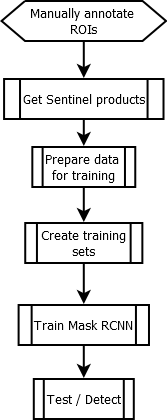
\includegraphics[width=.2\textwidth]{pics/overview.PNG}
  \caption{Gesamtablauf der Anwendung}
  \label{fig:overview}
\end{figure}
Zuerst müssen die Daten für das Training bzw. für die Erkennung manuell annotiert werden. Diese Metadaten werden dann genutzt, um automatisch Sentinelprodukte\footnote{Aufnahmenpakete der Sentinel-Plattformen werden als Produkte bezeichnet.} mittels einer API, die von der Copernicus zur Verfügung gestellt wird, herunterzuladen. Aus den Produkten werden die relevanten Bänder extrahiert und unter anderem die jeweiligen NDVI-Werte berechnet. Nachdem die Produkte für das Training vorbereitet wurden, werden die Daten in ein Trainings- und in ein Validierungsdatensatz aufgeteilt. Der folgende Trainingsprozess basiert auf diesen Datensätzen. Sobald das Training abgeschlossen ist, kann die Performanz des Modells getestet werden. 

\section{Annotation}\label{sec:annotation}

Zu Beginn werden die Regionen, die entweder für das Training benutzt oder überprüft werden, manuell erfasst. Vorrausgesetzte Informationen sind
\begin{itemize}
	\item Geografische Koordinaten,
	\item Zeitraum des Befalls und
	\item Bezeichnung der Infektion.
\end{itemize}
Als Format dieser Informationen dient \textit{GeoJSON}\footnote{GeoJSON ist eine Erweiterung des JSON-Format und beschreibt geografische Daten und Geometrien. GeoJSON wird durch den RFC7946-Standard definiert.}. GeoJSON enthält nicht nur geografische Daten, sondern ist auch um benutzerdefinierte Eigenschaften (\texttt{properties}) erweiterbar. Die Annotationen sind also GeoJSON-Features, die ein geografisches Polygon und Metadaten enthalten.

\begin{lstlisting}[language=json,caption={Annotation},captionpos=b]
{
  "type": "Feature",
  "properties": {
    "disease": 1,
    "from": "2018-07-12T13:00:00Z-7DAYS",
    "to": "2018-07-12T13:00:00Z+7DAYS"
  },
  "geometry": {
    "type": "Polygon",
    "coordinates": [[[11.171988617177981,44.574291380353003],
       [11.1726616444942,44.574017992242283],
       [11.17338129910439,44.575068359984279],
       [11.17273129334275,44.575299863118993],
       [11.171988617177981,44.574291380353003]]]
  }
}
\end{lstlisting}
\noindent
\texttt{properties.disease} enthält die eindeutige, nummerische Repräsentation der Klasse bzw. Krankheit, die in dieser Region enthalten ist. Die Zuordnung der nummerischen Werte und des textuellen Bezeichners werden in einer separaten JSON als Schlüssel-Wert-Paare konfiguiert, wobei der Schlüssel nummerisch und der Wert textuell ist. Hier ist, darauf zu achten, dass der Schlüssel $\ge1$ ist, da $0$ der implizite Schlüssel der Mask R-CNN-Implementierung für den Hintergrund ist. Diese Eigenschaft ist nur für das Training von Relevanz.
\\\\
\texttt{properties.from} und \texttt{properties.to} sind jeweils Start- und Endzeitpunkt, in dem nach verfügbaren Sentinelprodukten gesucht werden soll. Das Format der jeweiligen Eigenschaften kann eine der folgenden Formen haben\footnote{Die Formate basieren auf der \texttt{sentinelsat}-Version 0.12.2.}:
\begin{itemize}
	\item \texttt{yyyyMMdd}
	\item \texttt{yyyy-MM-ddThh:mm:ss.SSSZ} (ISO-8601)
	\item \texttt{yyyy-MM-ddThh:mm:ssZ}
	\item \texttt{NOW}
	\item \texttt{NOW-<n>DAY(S)} (oder \texttt{HOUR(S)}, \texttt{MONTH(S)}, usw.)
	\item \texttt{NOW+<n>DAY(S)}
	\item \texttt{yyyy-MM-ddThh:mm:ssZ-<n>DAY(S)}
	\item \texttt{NOW/DAY} (oder \texttt{HOUR}, \texttt{MONTH} usw.) - Der Wert wird auf den jeweiligen Typ (z.B. auf den Tag) gerundet.
\end{itemize}
\noindent
Es ist angebracht einen Zeitraum von mehreren Tagen bzw. Wochen zu wählen, da die Sentinel-2-Satelliten keine täglichen Daten liefern und weil eine Infektion typischerweise über einen längeren Zeitraum vorherrscht. Die Zeitspanne ist von der Krankheit abhängig. Hier wurden eine Woche vor und nach dem Aufnahmezeitpunkt genutzt, um nach Produkten zu suchen.

\section{Suche nach Sentinelprodukte}

\begin{figure}[ht]
  \centering
  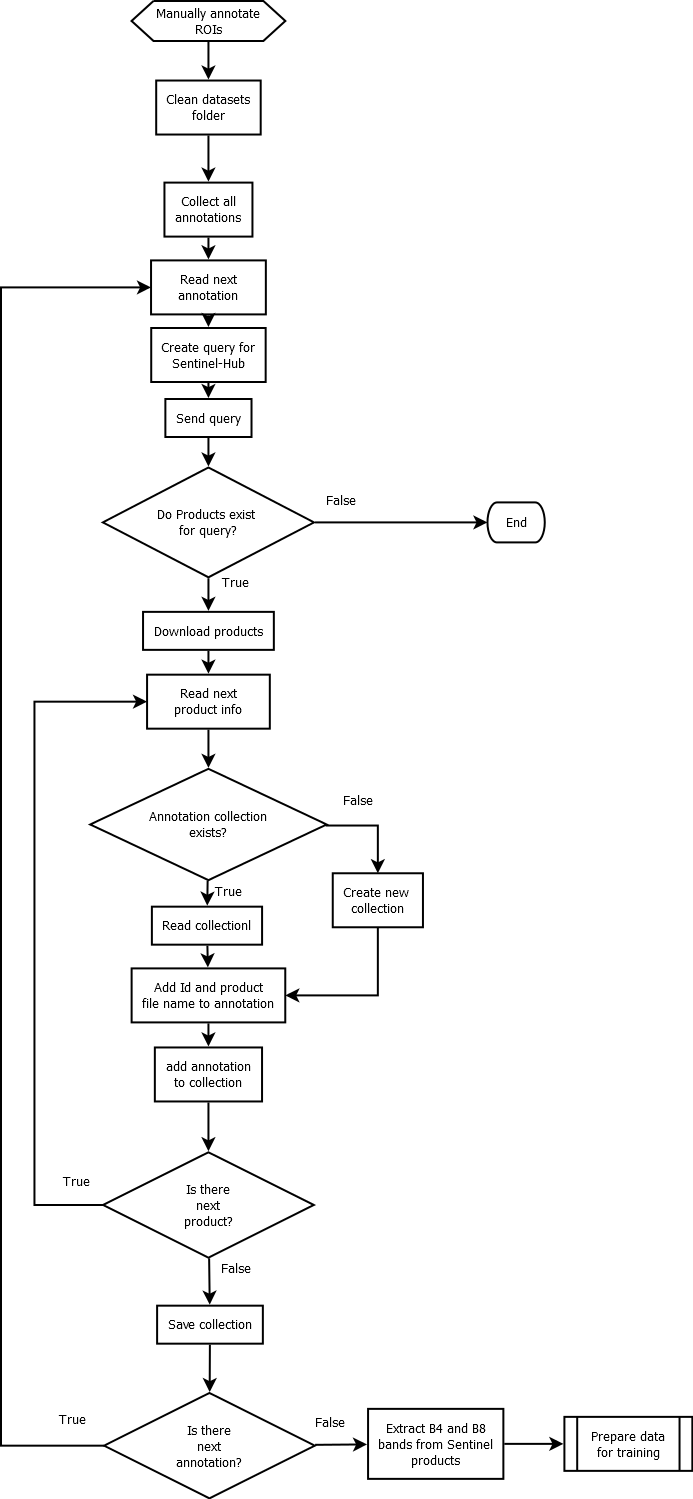
\includegraphics[height=\textheight]{pics/get-products.png}
  \caption{Ablaufdiagramm der Beschaffung der Sentinelprodukte}
  \label{fig:get-products}
\end{figure}

Der \textit{Copernicus Open Access Hub}\footnote{\url{https://scihub.copernicus.eu/}} ermöglicht freien und offenen Zugriff auf Sentinel-Produkte. Die Daten sind sowohl über eine grafische Oberfläche als auch über eine REST-API verfübar. Vorrausgesetzung für beide Optionen ist ein Account, der über die grafische Oberfläche erstellt werden kann.
\\\\
Die Nutzung der Schnittstelle erfolgt über die Python-Bibliothek \texttt{sentinelsat}\footnote{https://sentinelsat.readthedocs.io/en/stable}. Bei einer Anfrage müssen die GeoJSON-Dateien in WKT\footnote{WKT (Well-known text) ist eine Markup-Sprache zur Repräsentation von geometrischen Objekten auf Karten und räumlichen Referenzsystemen.} umgewandelt werden, was von der Bibliothek übernommen werden kann. Die WKT-Geometrie wird als \textit{footprint} (dt.: Fußabdruck) bezeichnet. Desweiteren wird der Plattformname statisch als `Sentinel-2' definiert, damit keine Produkte von den anderen Sentinelplattformen zurückgegeben werden. Der Suchzeitraum wird aus der jeweiligen GeoJSON-Datei übernommen. Sollten für die Suchanfragen keine Produkte existieren, wird die Anwendung beendet, da es keine Basis gibt, auf der das Netzwerk trainiert werden kann. Eventuell muss bei so einem Fall der Zeitraum erweitert und Prozess wiederholt werden. Bei vorhandenen Produkten lädt das Skript diese herunter. Die Produkte werden in einem komprimierten Format geliefert und enthalten neben zusätzlichen Informationen, Banddaten in separaten Dateien im JPEG2000-Format\footnote{JPEG 2000 genau wie GeoTIFF ist ein Bildformat in dem auch Metadaten abgelegt werden können. So sind Pixel geografischen Koordinaten zuordbar.}.
\\\\
Für jedes Produkt, das zur aktuellen Annotation gehört, wird ein neuer Eintrag zu einer \textit{FeatureCollection} hinzugefügt. Zusätzlich wird eine \textit{UUID} (Universally Unique Identifier) generiert und zusammen mit dem Dateinamen der Produktes in den Metadaten gespeichert. Für die spätere Entwicklung sind die Annotationen leichter zu finden und bearbeitbar. Außerdem bleiben dadurch die Originaldaten unberührt. Dieser Schritt wird für jede vorhandene Annotationsdatei wiederholt. Anschließend werden die Bilddateien für B4 und B8 aus dem Produkt extrahiert.

\section{Aufbereitung der Sentineldaten}
\chapter{Overfitting}\label{chap:overfitting}

\section{Begriffserklärung}\label{sec:what-is-overfitting}

Genaue Daten über Krankheitsbefälle im Agrarsektor sind rar, da diese in der Regel nicht öffentlich zugänglich sind.\footnote{Datenschutz kann ein Grund dafür sein.}  Daher musste mit \textit{Overfitting} gerechnet werden. Das künstliche neurale Netzwerk soll daraufhin trainiert werden, dass es möglichst alle Befälle, die untersucht werden, erkennt. Dafür wird es im ersten Schritt mit einem Trainingsdatensatz trainiert. Im folgenden Schritt mit einem kleineren Validierungsdatensatz überprüft, wie gut das Netz trainiert wird. Overfitting tritt auf, wenn das Netz auf die Daten aus dem Trainingsdatensatz mit sehr hoher Erfolgsquote erkennt, jedoch vergleichsweise schlechte Ergebnisse bei der Validierung bzw. bei unbekannten Daten erzielt. 
\\\\
\begin{figure}[ht]
  \centering
  
\includegraphics[height=2.5cm]{pics/mask.png}
  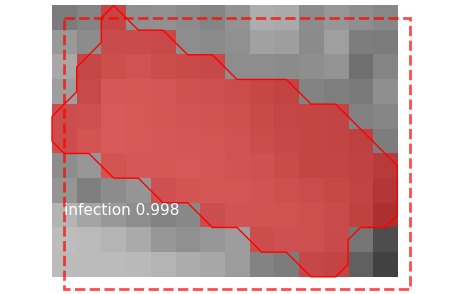
\includegraphics[height=2.5cm]{pics/pred.png}
  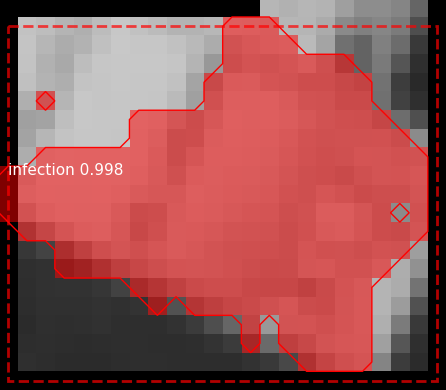
\includegraphics[height=2.5cm]{pics/bad-pred.png}
  \caption[Beispiel Overfitting]{V.l.n.r. Bild von infizierter Agrarfläche aus Trainingsdatensatz / Binärmaske der inifizierten Region, wird gemeinsam mit dem linken Bild zum Training in das KNN gespeist / Selbiges Bild, Ergebnis nach Trainingsdurchlauf, prognostizierte Ergebnisfläche in rot / Bild der selben Fläche, was nicht aus dem Trainingsdatensatz stammt, prognostizierte Ergebnisfläche in rot}
  \label{fig:example-overfitting}
\end{figure}
\noindent
\todo{Erwähnen, dass Mask RCNN Bild und Masken für Training benötigt.}
In Abb. \ref{fig:example-overfitting} ist ein Beispiel wie Overfitting sich auswirken kann. Die linken zwei Bilder sind ein exemplarischer Auszug aus dem Trainingsdatensatz. Einmal eine visuelle Repräsentation der NDVI-Werte der infizierten Agrarfläche und die Binärmaske, welche die infizierte Fläche markiert. Das selbe Bild wurde nach einem erfolgreichen Trainingsdurchlauf der Mask R-CNN-Implementierung übergeben und es hat den erkrankten Bereich nahezu perfekt erkannt. Das vierte Bild zeigt zentriert das selbe Feld. Jedoch ist der Ausschnitt größer, rotiert und die Aufnahme stammt von einem anderen Datum.\todo{Genaues Datum nötig?} Der Prognose zur Folge ist die Infizierung auf die benachbarten Felder übergesprungen, was nicht der Wahrheit entspricht. Overfitting ist ein bekanntes Problem im Bereich des maschinellen Lernens und es existieren multiple Methoden, um dem entgegenzuwirken.

% ----- Abbildungen ----- %
%\addcontentsline{toc}{section}{Abbildungsverzeichnis} % falls in Inhalsverzeichnis
%\listoffigures

% ----- Tabellen----- %
% \addcontentsline{toc}{section}{Tabellenverzeichnis}  % falls in Inhalsverzeichnis
% \fancyhead[L]{Abbildungsverzeichnis / Abkürzungsverzeichnis} %Kopfzeile linksx
% \listoftables

% ----- Listings ----- %
% Listingverzeichnis soll im Inhaltsverzeichnis auftauchen
%\addcontentsline{toc}{section}{Listingverzeichnis}
%\fancyhead[L]{Abbildungs- / Tabellen- / Listingverzeichnis} %Kopfzeile links
%\renewcommand{\lstlistlistingname}{Listingverzeichnis}
%\lstlistoflistings

\pagestyle{plain} % zurueck setzen von roemische seitenanzahl


%\printbibliography
\bibliographystyle{abbrv}
\bibliography{literature}
	
% ----- Listings ----- %

%\chapter*{Erklärung}
\addcontentsline{toc}{chapter}{Erklärung}

Ich versichere, dass ich die vorliegende Arbeit selbstständig und nur unter Verwendung der angegebenen Quellen und Hilfsmittel angefertigt habe, insbesondere sind wörtliche oder sinngemäße Zitate als solche gekennzeichnet. Mir ist bekannt, dass Zuwiderhandlung auch nachträglich zur Aberkennung des Abschlusses führen kann.\\\\
Ich versichere, dass das elektronische Exemplar mit den gedruckten Exemplaren übereinstimmt.
\\\\\\
Ort:\hspace{3cm}Datum:\hspace{3cm}Unterschrift:

\end{document}